%!TEX program = xelatex
% 完整编译: xelatex -> biber/bibtex -> xelatex -> xelatex
\documentclass[lang=cn,11pt,a4paper]{elegantpaper}

\title{python中的数据爬取}
\author{杨晨 \\学号2021212171}
\institute{北京邮电大学 计算机学院}

% \version{0.10}
\date{\zhtoday}

% 本文档命令
\usepackage{array}
\usepackage{xcolor}
\newcommand{\ccr}[1]{\makecell{{\color{#1}\rule{1cm}{1cm}}}}

% 设置全局代码样式
\lstset{
  language=Python, % 设置语言为Python
  keywordstyle=\color{blue}, % 设置关键字颜色为蓝色
  commentstyle=\color{green!60!black}, % 设置注释颜色为绿色
  stringstyle=\color{orange}, % 设置字符串颜色为橙色
  showstringspaces=false, % 不显示字符串中的空格
  frame=single, % 添加边框
  breaklines=true, % 自动断行
  numberstyle=\tiny\color{gray}, % 设置行号样式为小号灰色
  captionpos=b % 设置标题位置为底部
}

\lstdefinelanguage{text}{
    showstringspaces=false,
    breaklines=true,
    breakatwhitespace=true,
    tabsize=4
}

\begin{document}



\maketitle
% \tableofcontents

\section{概述}

\subsection{实验内容}

\begin{enumerate}

    \item 爬取学堂在线的计算机类课程页面内容

    \url{https://www.xuetangx.com/search?query=&org=&classify=1&type=&status=&page=1}
    
    要求将课程名称、老师、所属学校和选课人数信息,保存到一个csv文件中。
    
    \item 爬取链家官网二手房的数据 
    
    \url{https://bj.lianjia.com/ershoufang/}
    
    要求爬取北京市东城、西城、海淀和朝阳四个城区的数据(每个区爬取5页),将楼盘名称、总价、平米数、单价保存到json文件中。
\end{enumerate}

\subsection{开发环境}

\begin{itemize}
    \item Windows10
    \item PyCharm 2023.2.4 (Professional Edition)
\end{itemize}

\section{实验过程}

\subsection{学堂在线计算机类课程内容爬取}

\subsubsection{介绍}

首先,按照PPT上的方法,用静态页面的方式进行爬取,但是发现爬虫关闭后,也没有爬取到任何数据

考虑网页是动态加载的,进入网页审查,发现以下结果
\clearpage

\begin{figure}[!htb]
\centering
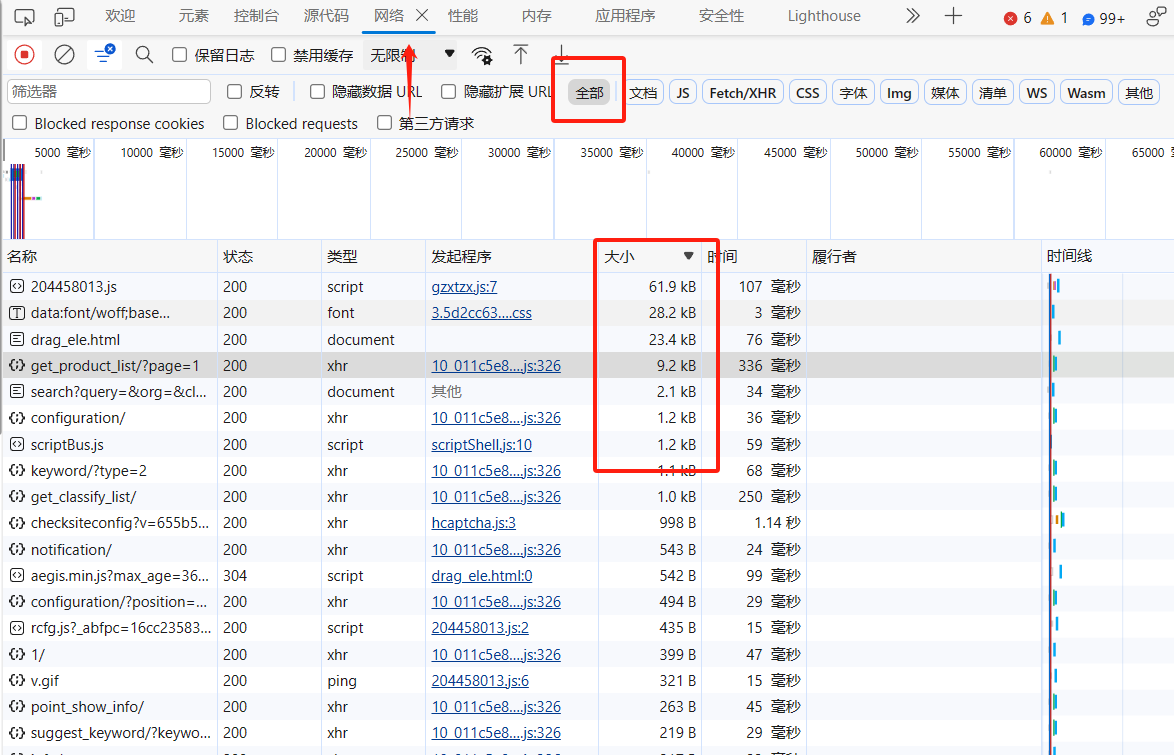
\includegraphics[width=0.9\textwidth]{1.png}
\end{figure}

现在明确确实是动态页面。

然后进一步发现是Ajax类型,以下为截图

\begin{figure}[!htb]
\centering
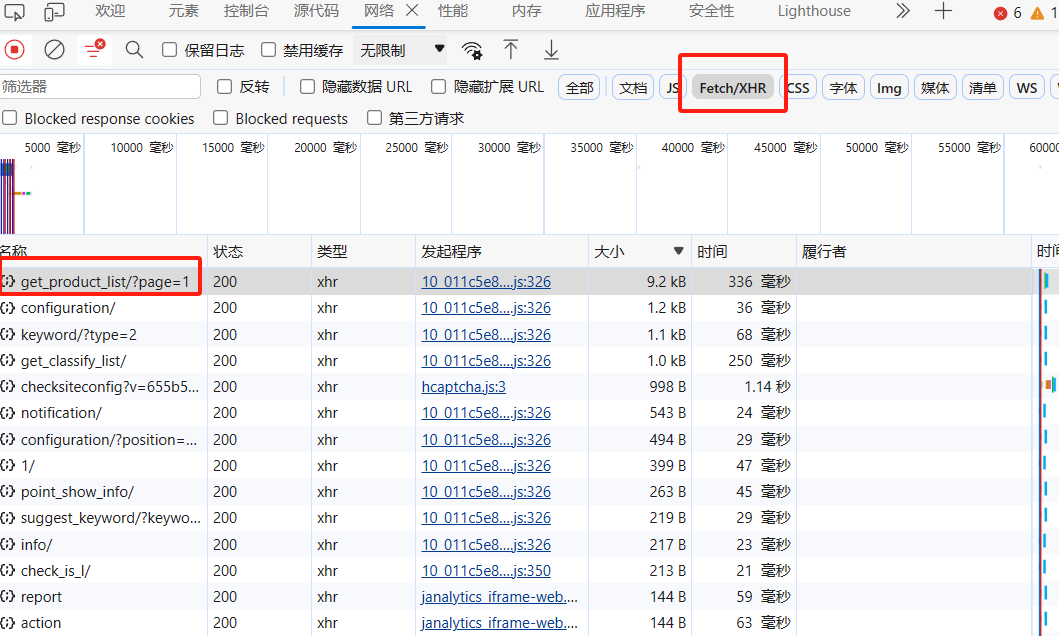
\includegraphics[width=0.9\textwidth]{2.png}
\end{figure}

点击打开page里的product\_lists可以看见课程的相关信息,正是我们需要爬取的内容,如下所示
\clearpage

\begin{figure}[!htb]
\centering
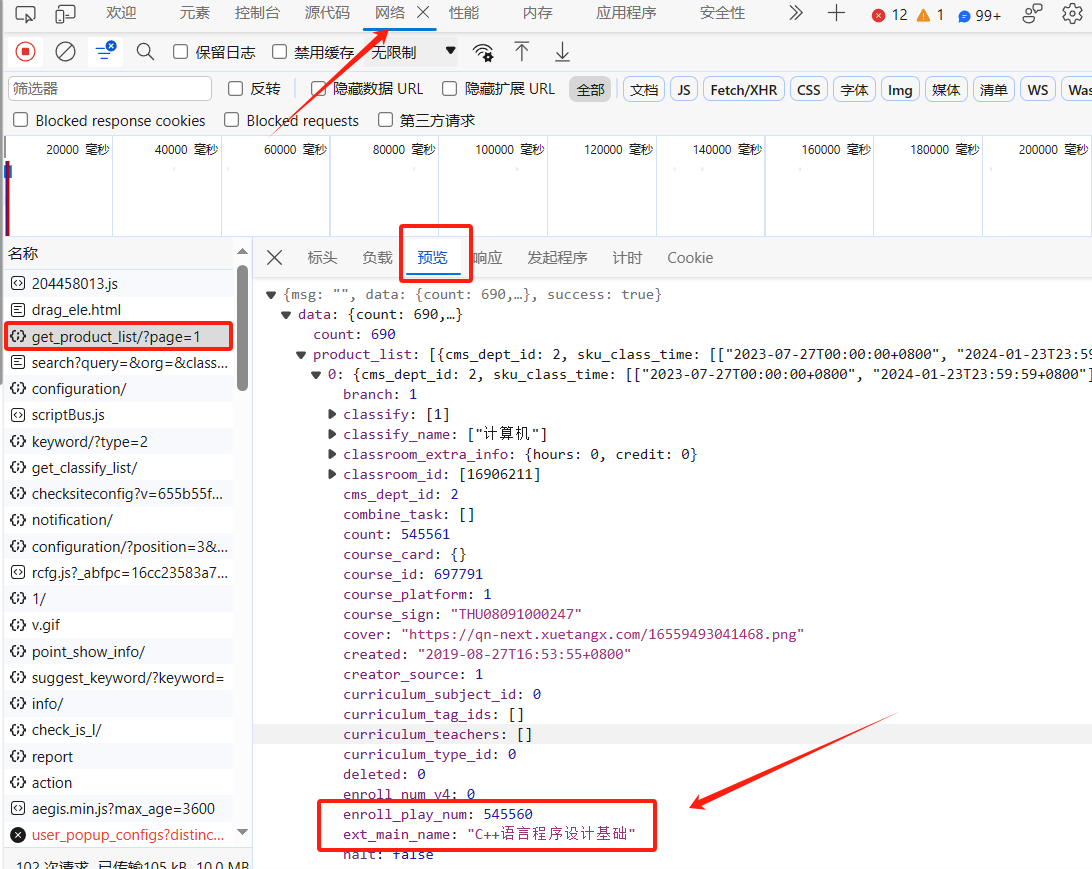
\includegraphics[width=0.9\textwidth]{3.png}
\end{figure}

基于以上的发现明确进行动态页面的爬取

\subsubsection{爬取方法}

\begin{enumerate}
    \item 找到爬取的链接以及请求的方式
    \begin{figure}[!htb]
    \centering
    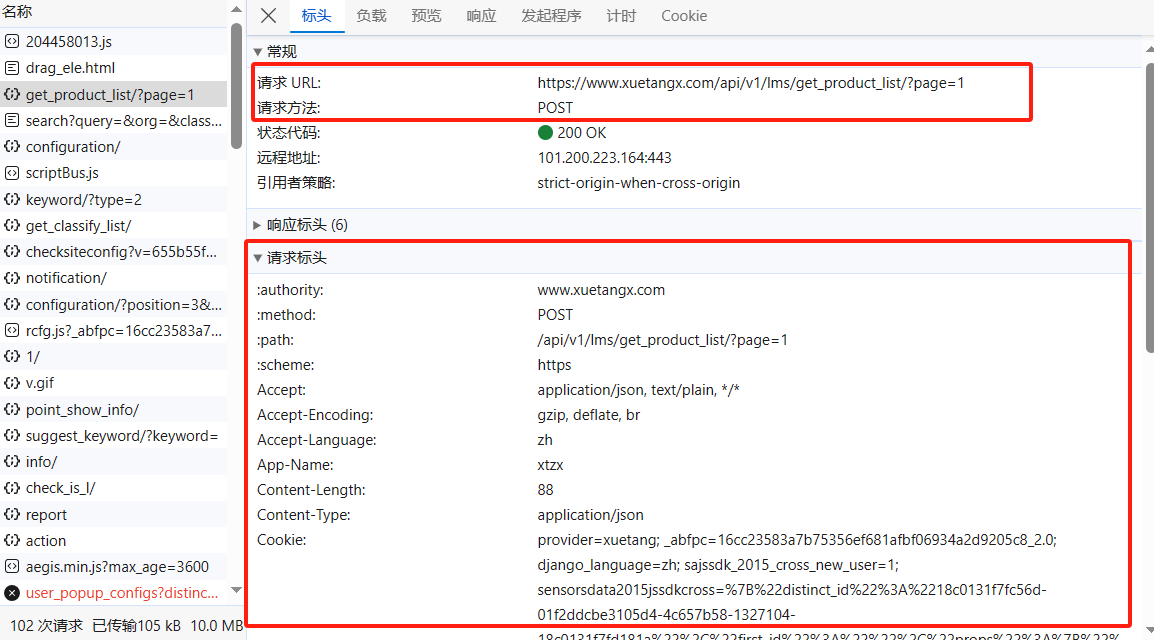
\includegraphics[width=0.9\textwidth]{4.png}
    \end{figure}
    \item 构造header,找到Headers选项,查看请求头
    \item 将此代码赋值下来,填充headers的构造,代码如下所示
    \begin{lstlisting}
# 请求头
headers = {
    "authority": "www.xuetangx.com",
    "method": "POST",
    "scheme": "https",
    "accept": "application/json, text/plain, */*",
    "accept-encoding": "gzip, deflate, br",
    "accept-language": "zh",
    "content-type": "application/json",
    "cookie": "provider=xuetang; django_language=zh",
    "django-language": "zh",
    "origin": "https://www.xuetangx.com",
    "Referer": "https://www.xuetangx.com/search?query=&org=&classify=1&type=&status=&page=1",
    "sec-fetch-dest": "empty",
    "sec-fetch-mode": "cors",
    "sec-fetch-site": "same-origin",
    "user-agent": "Mozilla/5.0 (Windows NT 10.0; Win64; x64) AppleWebKit/537.36 "
    "(KHTML, like Gecko) Chrome/119.0.0.0 Safari/537.36",
    "X-Client": "web",
    "Xtbz": "xt",
}
    \end{lstlisting}
    \item 除了请求头此外,还需要post的提交表格数据
    \begin{figure}[!htb]
    \centering
    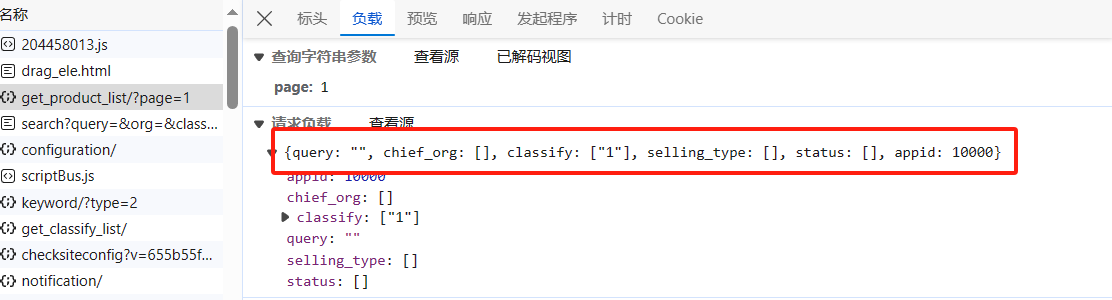
\includegraphics[width=0.9\textwidth]{5.png}
    \end{figure}

    代码如下
    \begin{lstlisting}
data = {
    "query": "",
    "chief_org": [],
    "classify": ["1"],
    "selling_type": [],
    "status": [],
    "appid": 10000,
}
    \end{lstlisting}
    \item 在前面第一步已经分析,采取的是post的页面的请求方法,那么借助\lstinline{FormRequest}函数即可实现post请求。重写\lstinline{tart_request(self)}函数,然后经过这个函数不断的循环发送请求,该函数代码实现如下
    \begin{lstlisting}
def start_requests(self):
    for page_num in range(1, 70):
        yield scrapy.FormRequest(
            url="https://www.xuetangx.com/api/v1/lms/get_product_list/?page={}".format(
                page_num
            ),
            headers=self.headers,
            method="POST",
            body=json.dumps(self.data),
            callback=self.parse,
        )
    \end{lstlisting}
    \item 接着就是解析内容的阶段根据我们的需求,需要爬取课程名称,老师,所属学校以及课程人数,那么将items.py文件如下实现:
    \begin{lstlisting}
class XuetangxItem(scrapy.Item):
    # 课程名称、教师、学校、学生人数
    course_name = scrapy.Field()
    teacher = scrapy.Field()
    school = scrapy.Field()
    student_num = scrapy.Field()
    \end{lstlisting}
    \item 那么对于response返回的内容,使用json.loads处理获取到的json文件,json.loads()函数是将json格式数据转换为字典。网页product\_list部分显示如下:
    \begin{figure}[!htb]
    \centering
    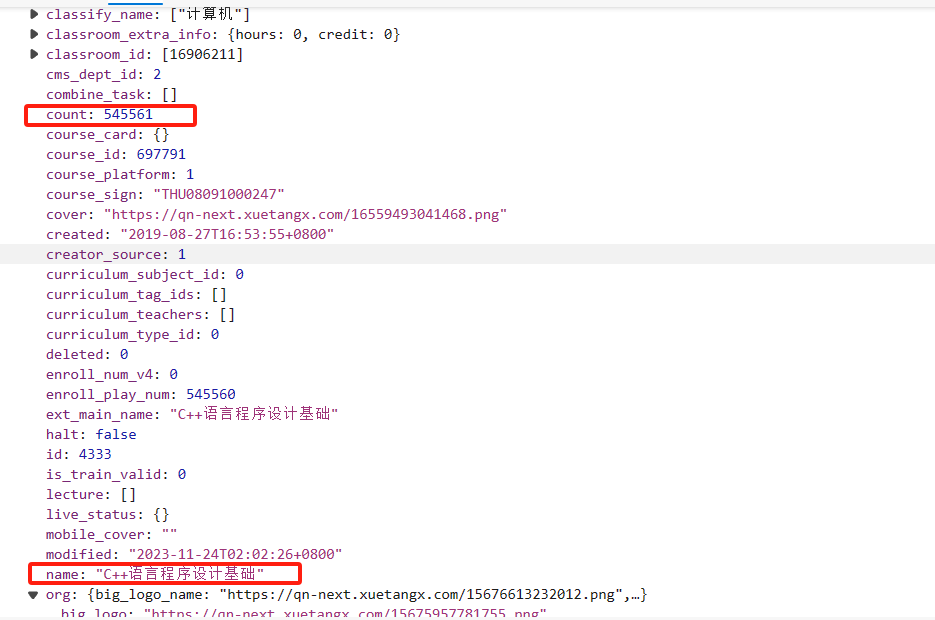
\includegraphics[width=0.9\textwidth]{6.png}
    \end{figure}
    
    那么对进行product\_list内容如下方式进行提取
    \begin{lstlisting}
def parse(self, response):
    for product in json.loads(response.body)["data"]["product_list"]:
        item = XuetangxItem()
        item["course_name"] = "课程名称:" + product["name"]
        item["teacher"] = "课程讲师:"
        for teacher in product["teacher"]:  # 一个课程可能有多个讲师
            item["teacher"] += teacher["name"] + " "
        item["school"] = "开课学校:" + product["org"]["name"]
        item["student_num"] = "学生人数:" + str(product["count"])
    \end{lstlisting}
    \item 然后pipelines进行将数据写入csv文件,那么pipelines.py文件如下所示
    \begin{lstlisting}
import csv

class XuetangxPipeline:
    def __init__(self):
        self.file = open('XuetangxData.csv', 'w+', encoding='utf-8', newline='')
        self.writer = csv.writer(self.file)

    def process_item(self, item, spider):
        self.writer.writerow([item['course_name'], item['teacher'], item['school'], item['student_num']])
        return item

    def close_spider(self, spider):
        self.file.close()
    \end{lstlisting}
    \item 最后当然需要将管道打开,那么settings.py文件如下所示
    \begin{lstlisting}
ROBOTSTXT_OBEY = False
# ITEM_PIPELINES = {'myproject.pipelines.MyPipeline': 300}

ITEM_PIPELINES = {'myproject.pipelines.XuetangxPipeline': 300}
    \end{lstlisting}
\end{enumerate}

\subsubsection{爬取结果}

\clearpage

\begin{figure}[!htb]
    \centering
    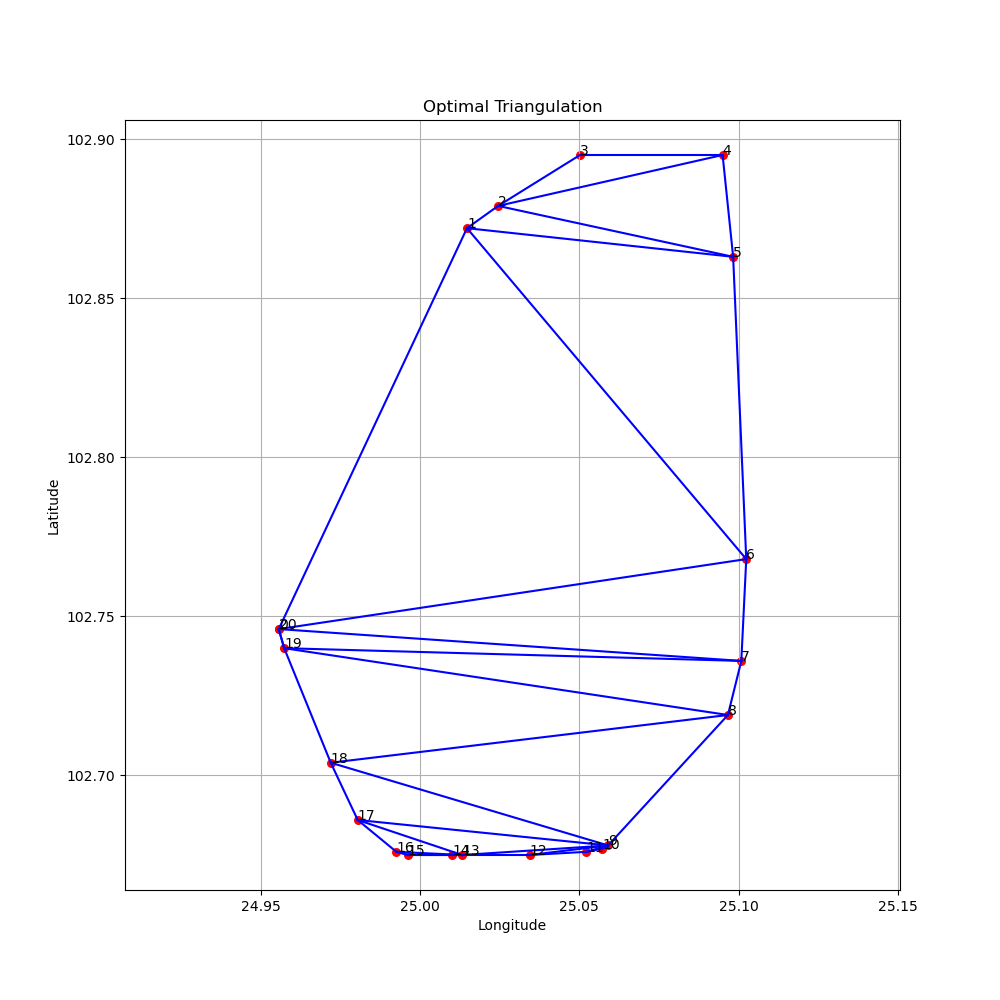
\includegraphics[width=0.9\textwidth]{result1.png}
    \caption{学堂在线爬取结果}
    \label{fig:enter-label}
\end{figure}

\subsection{链家官网北京二手房数据爬取}

\subsubsection{介绍}
链家的官网是静态页面,相比之下要容易处理

审查页面,找到想提取的楼盘名称、总价、平米数、单价的xpath,进行提取即可

此外,对于第1页,第2页,网页的url具有相似特征/pg1,/pg2;这使得爬取较为方便

\subsubsection{爬取方法}

\begin{enumerate}
    \item 构造spider
    \begin{lstlisting}
class LianjiaSpider(scrapy.spiders.Spider):
    name = "lianjia"
    allowed_domains = ["lianjia.com"]
    start_urls = [
        "https://bj.lianjia.com/ershoufang/dongcheng/pg1/",
        "https://bj.lianjia.com/ershoufang/xicheng/pg1/",
        "https://bj.lianjia.com/ershoufang/chaoyang/pg1/",
        "https://bj.lianjia.com/ershoufang/haidian/pg1/",
    ]
    \end{lstlisting}
    \item 需要爬取的信息有:楼盘名称、总价、平米数、单价。那么items.py中的代码如下
    \begin{lstlisting}
class LianjiaItem(scrapy.Item):
    # 楼盘名称、总价、平米数、单价
    name = scrapy.Field()
    price = scrapy.Field()
    area = scrapy.Field()
    unit_price = scrapy.Field()

    \end{lstlisting}
    \item 审查页面,筛选想提取的信息,如下
    \begin{figure}[!htb]
    \centering
    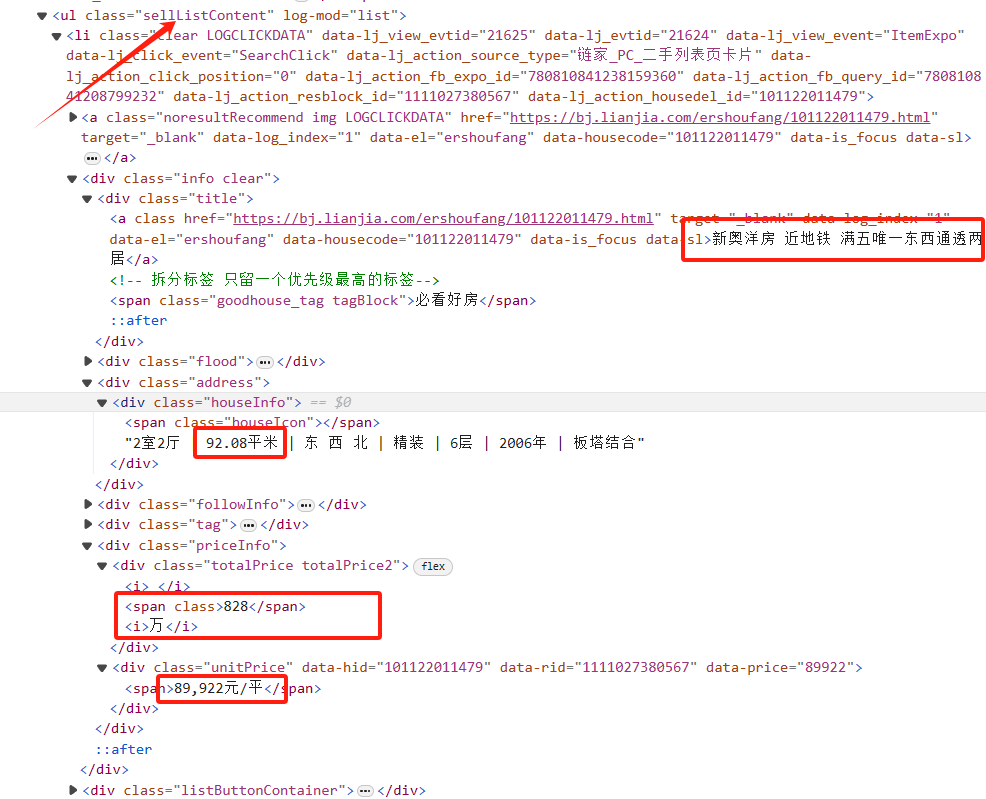
\includegraphics[width=0.9\textwidth]{7.png}
    \end{figure}
    
    在每个sellListContent类下面,每个li代表一个房子的信息。进行提取的代码如下
    \begin{lstlisting}
def parse(self, response):
    item = LianjiaItem()
    distinct = response.url.split("/")[4]
    page = response.url.split("/")[5]
    for each in response.xpath('//ul[@class="sellListContent"]/li'):
        item["name"] = "楼盘名称:" + each.xpath("div/div/a/text()").get()
        price_value = each.xpath(
            "div/div[@class='priceInfo']/div[@class='totalPrice totalPrice2']/span/text()"
        ).get()
        price_unit = each.xpath(
            "div/div[@class='priceInfo']/div[@class='totalPrice totalPrice2']/i[last()]/text()"
        ).get()
        item["price"] = "总价:" + f"{price_value}{price_unit}"
        area_text = each.xpath(
            ".//div[@class='address']/div[@class='houseInfo']/text()"
        ).get()
        match = re.search(r"(\d+(\.\d+)?)平米", area_text)
        if match:
            item["area"] = "平米数:" + match.group(1) + "平米"
        else:
            item["area"] = "平米数:" + "unknown"
        item["unit_price"] = "单价:" + each.xpath(
            "div/div[@class='priceInfo']/div[@class='unitPrice']/span/text()"
        ).get()
        if item["name"] and item["price"] and item["area"] and item["unit_price"]:
            yield item
    \end{lstlisting}
    为了便于提取平米数,使用了正则表达式re库
    \item 因为需要提取前5页的内容,所以需要构造下一页的URL,并发送一个新的请求,回调函数为自身的\lstinline{parse}方法,实现翻页功能
    \begin{lstlisting}
if page != "pg5":
    next_page = int(page[2]) + 1
    next_url = "https://bj.lianjia.com/ershoufang/{}/pg{}/".format(distinct, next_page)
    yield scrapy.Request(next_url, callback=self.parse)
    \end{lstlisting}
    \item 然后pipelines进行将数据写入json文件,那么pipelines.py文件如下所示
    \begin{lstlisting}
class LianjiaPipeline:
    def __init__(self):
        self.file = open("LianjiaData.json", "w+", encoding="utf-8")
        self.writer = csv.writer(self.file)

    def process_item(self, item, spider):
        dict_item = dict(item)
        json_str = json.dumps(dict_item, ensure_ascii=False) + "\n"
        self.file.write(json_str)
        return item

    def close_spider(self, spider):
        self.file.close()
    \end{lstlisting}
    \item 最后需要将管道打开,那么settings.py文件如下所示
    \begin{lstlisting}
ROBOTSTXT_OBEY = False
# ITEM_PIPELINES = {'myproject.pipelines.MyPipeline': 300}

# ITEM_PIPELINES = {'myproject.pipelines.XuetangxPipeline': 300}

ITEM_PIPELINES = {'myproject.pipelines.LianjiaPipeline': 300}
    \end{lstlisting}
\end{enumerate}

\clearpage

\subsubsection{爬取结果}

\begin{figure}[!htb]
    \centering
    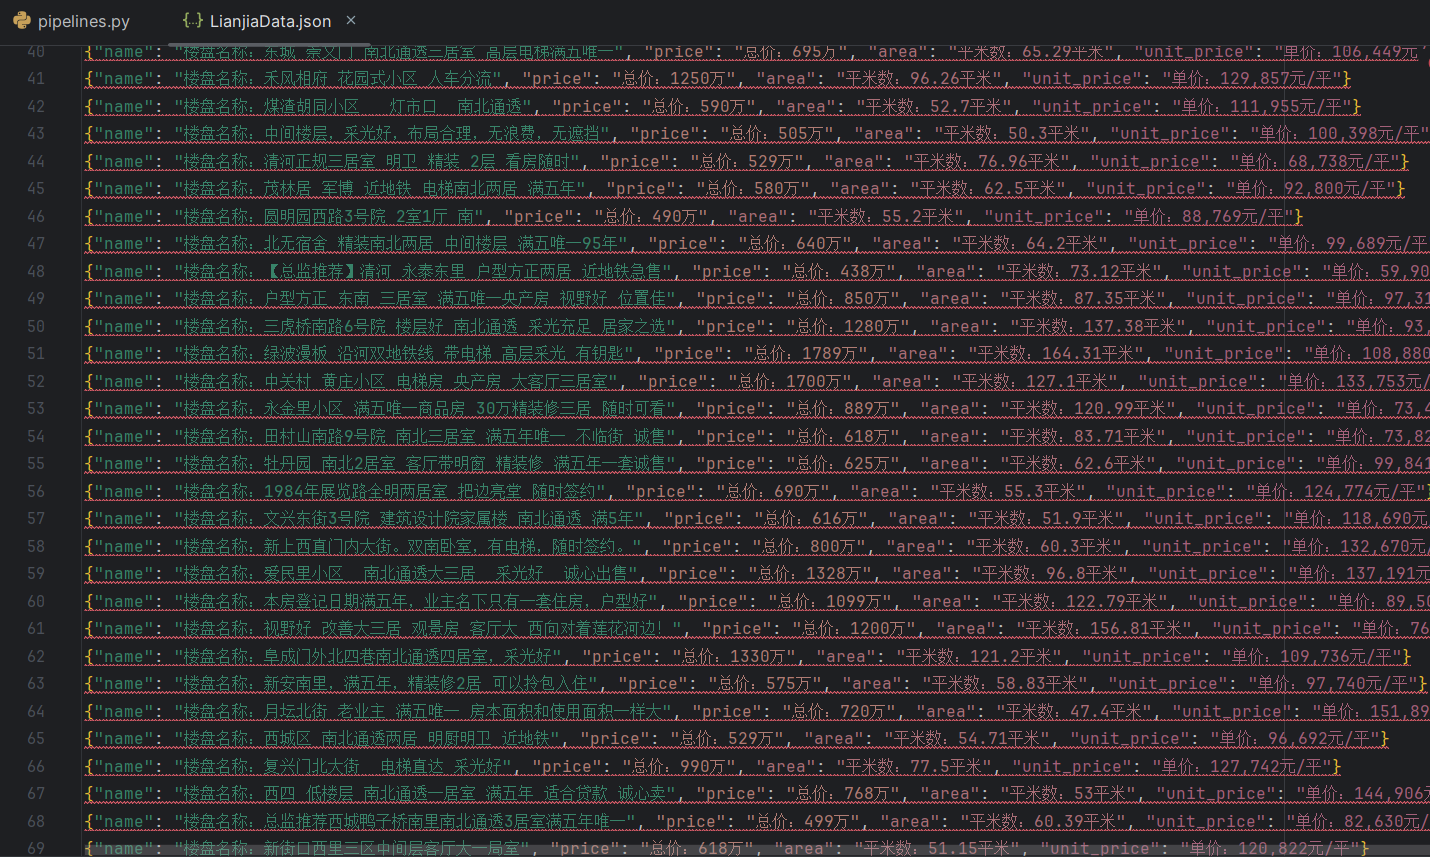
\includegraphics[width=0.9\textwidth]{result2.png}
    \caption{链家爬取结果}
    \label{fig:enter-label}
\end{figure}

\section{附录:spider.py完整代码}

\subsection{爬取学堂在线}
\begin{lstlisting}
import scrapy
from ..items import XuetangxItem
import json


class XuetangxSpider(scrapy.spiders.Spider):
    name = "xuetangx"
    allowed_domains = ["xuetangx.com"]
    # 请求头
    headers = {
        "authority": "www.xuetangx.com",
        "method": "POST",
        "scheme": "https",
        "accept": "application/json, text/plain, */*",
        "accept-encoding": "gzip, deflate, br",
        "accept-language": "zh",
        "content-type": "application/json",
        "cookie": "provider=xuetang; django_language=zh",
        "django-language": "zh",
        "origin": "https://www.xuetangx.com",
        "Referer": "https://www.xuetangx.com/search?query=&org=&classify=1&type=&status=&page=1",
        "sec-fetch-dest": "empty",
        "sec-fetch-mode": "cors",
        "sec-fetch-site": "same-origin",
        "user-agent": "Mozilla/5.0 (Windows NT 10.0; Win64; x64) AppleWebKit/537.36 "
        "(KHTML, like Gecko) Chrome/119.0.0.0 Safari/537.36",
        "X-Client": "web",
        "Xtbz": "xt",
    }
    data = {
        "query": "",
        "chief_org": [],
        "classify": ["1"],
        "selling_type": [],
        "status": [],
        "appid": 10000,
    }
    download_delay = 1

    def start_requests(self):
        for page_num in range(1, 70):
            yield scrapy.FormRequest(
                url="https://www.xuetangx.com/api/v1/lms/get_product_list/?page={}".format(
                    page_num
                ),
                headers=self.headers,
                method="POST",
                body=json.dumps(self.data),
                callback=self.parse,
            )

    def parse(self, response):
        for product in json.loads(response.body)["data"]["product_list"]:
            item = XuetangxItem()
            item["course_name"] = "课程名称:" + product["name"]
            item["teacher"] = "课程讲师:"
            for teacher in product["teacher"]:  # 一个课程可能有多个讲师
                item["teacher"] += teacher["name"] + " "
            item["school"] = "开课学校:" + product["org"]["name"]
            item["student_num"] = "学生人数:" + str(product["count"])

            if (
                item["course_name"]
                and item["teacher"]
                and item["school"]
                and item["student_num"]
            ):
                yield item

\end{lstlisting}

\subsection{爬取链家}

\begin{lstlisting}
import scrapy
from ..items import LianjiaItem
import re


class LianjiaSpider(scrapy.spiders.Spider):
    name = "lianjia"
    allowed_domains = ["lianjia.com"]
    start_urls = [
        "https://bj.lianjia.com/ershoufang/dongcheng/pg1/",
        "https://bj.lianjia.com/ershoufang/xicheng/pg1/",
        "https://bj.lianjia.com/ershoufang/chaoyang/pg1/",
        "https://bj.lianjia.com/ershoufang/haidian/pg1/",
    ]

    def parse(self, response):
        item = LianjiaItem()
        distinct = response.url.split("/")[4]
        page = response.url.split("/")[5]
        for each in response.xpath('//ul[@class="sellListContent"]/li'):
            item["name"] = "楼盘名称:" + each.xpath("div/div/a/text()").get()
            price_value = each.xpath(
                "div/div[@class='priceInfo']/div[@class='totalPrice totalPrice2']/span/text()"
            ).get()
            price_unit = each.xpath(
                "div/div[@class='priceInfo']/div[@class='totalPrice totalPrice2']/i[last()]/text()"
            ).get()
            item["price"] = "总价:" + f"{price_value}{price_unit}"
            area_text = each.xpath(
                ".//div[@class='address']/div[@class='houseInfo']/text()"
            ).get()
            match = re.search(r"(\d+(\.\d+)?)平米", area_text)
            if match:
                item["area"] = "平米数:" + match.group(1) + "平米"
            else:
                item["area"] = "平米数:" + "unknown"
            item["unit_price"] = "单价:" + each.xpath(
                "div/div[@class='priceInfo']/div[@class='unitPrice']/span/text()"
            ).get()
            if item["name"] and item["price"] and item["area"] and item["unit_price"]:
                yield item

        if page != "pg5":
            next_page = int(page[2]) + 1
            next_url = "https://bj.lianjia.com/ershoufang/{}/pg{}/".format(distinct, next_page)
            yield scrapy.Request(next_url, callback=self.parse)

\end{lstlisting}

% \subsection{全局选项}
% 此模板定义了一个语言选项 \lstinline{lang},可以选择英文模式 \lstinline{lang=en}(默认)或者中文模式 \lstinline{lang=cn}。当选择中文模式时,图表的标题引导词以及参考文献,定理引导词等信息会变成中文。你可以通过下面两种方式来选择语言模式:
% \begin{lstlisting}
% \documentclass[lang=cn]{elegantpaper} % or
% \documentclass{cn}{elegantpaper} 
% \end{lstlisting}

% \textbf{注意:} 英文模式下,由于没有添加中文宏包,无法输入中文。如果需要输入中文,可以通过在导言区引入中文宏包 \lstinline{ctex} 或者加入 \lstinline{xeCJK} 宏包后自行设置字体。 
% \begin{lstlisting}
% \usepackage[UTF8,scheme=plain]{ctex}
% \end{lstlisting}

% \subsection{数学字体选项}

% 本模板定义了一个数学字体选项(\lstinline{math}),可选项有三个:
% \begin{enumerate}
%   \item \lstinline{math=cm}(默认),使用 \LaTeX{} 默认数学字体(推荐,无需声明);
%   \item \lstinline{math=newtx},使用 \lstinline{newtxmath} 设置数学字体(潜在问题比较多)。
%   \item \lstinline{math=mtpro2},使用 \lstinline{mtpro2} 宏包设置数学字体,要求用户已经成功安装此宏包。
% \end{enumerate}

% \subsection{中文字体选项}

% 模板提供中文字体选项 \lstinline{chinesefont},可选项有
% \begin{enumerate}
%   \item \lstinline{ctexfont}:默认选项,使用 \lstinline{ctex} 宏包根据系统自行选择字体,可能存在字体缺失的问题,更多内容参考 \lstinline{ctex} 宏包\href{https://ctan.org/pkg/ctex}{官方文档}\footnote{可以使用命令提示符,输入 \lstinline{texdoc ctex} 调出本地 \lstinline{ctex} 宏包文档}。
%   \item \lstinline{founder}:方正字体选项(\textbf{需要安装方正字体}),后台调用 \lstinline{ctex} 宏包并且使用 \lstinline{fontset=none} 选项,然后设置字体为方正四款免费字体,方正字体下载注意事项见后文,用户只需要安装方正字体即可使用该选项。
%   \item \lstinline{nofont}:后台会调用 \lstinline{ctex} 宏包并且使用 \lstinline{fontset=none} 选项,不设定中文字体,用户可以自行设置中文字体,具体见后文。
% \end{enumerate}

% \subsubsection{方正字体选项}
% 由于使用 \lstinline{ctex} 宏包默认调用系统已有的字体,部分系统字体缺失严重,因此,用户希望能够使用其它字体,我们推荐使用方正字体。方正的{\songti 方正书宋}、{\heiti 方正黑体}、{\kaishu 方正楷体}、{\fangsong 方正仿宋}四款字体均可免费试用,且可用于商业用途。用户可以自行从\href{http://www.foundertype.com/}{方正字体官网}下载此四款字体,在下载的时候请\textbf{务必}注意选择 GBK 字符集,也可以使用 \href{https://www.latexstudio.net/}{\LaTeX{} 工作室}提供的\href{https://pan.baidu.com/s/1BgbQM7LoinY7m8yeP25Y7Q}{方正字体,提取码为:njy9} 进行安装。安装时,{\kaishu Win 10 用户请右键选择为全部用户安装,否则会找不到字体。}

% \begin{figure}[!htb]
% \centering
% 
\includegraphics[width=0.9\textwidth]{founder.png}
% \end{figure}

% \subsubsection{其他中文字体}
% 如果你想完全自定义字体\footnote{这里仍然以方正字体为例。},你可以选择 \lstinline{chinesefont=nofont},然后在导言区设置即可,可以参考下方代码:
% \begin{lstlisting}
% \setCJKmainfont[BoldFont={FZHei-B01},ItalicFont={FZKai-Z03}]{FZShuSong-Z01}
% \setCJKsansfont[BoldFont={FZHei-B01}]{FZKai-Z03}
% \setCJKmonofont[BoldFont={FZHei-B01}]{FZFangSong-Z02}
% \setCJKfamilyfont{zhsong}{FZShuSong-Z01}
% \setCJKfamilyfont{zhhei}{FZHei-B01}
% \setCJKfamilyfont{zhkai}[BoldFont={FZHei-B01}]{FZKai-Z03}
% \setCJKfamilyfont{zhfs}[BoldFont={FZHei-B01}]{FZFangSong-Z02}
% \newcommand*{\songti}{\CJKfamily{zhsong}}
% \newcommand*{\heiti}{\CJKfamily{zhhei}}
% \newcommand*{\kaishu}{\CJKfamily{zhkai}}
% \newcommand*{\fangsong}{\CJKfamily{zhfs}}
% \end{lstlisting}



% \subsection{自定义命令}
% 此模板并没有修改任何默认的 \LaTeX{} 命令或者环境\footnote{目的是保证代码的可复用性,请用户关注内容,不要太在意格式,这才是本工作论文模板的意义。}。另外,我自定义了 4 个命令:
% \begin{enumerate}
%   \item \lstinline{\email}:创建邮箱地址的链接,比如 \email{ddswhu@outlook.com};
%   \item \lstinline{\figref}:用法和 \lstinline{\ref} 类似,但是会在插图的标题前添加 <\textbf{图 n}> ;
%   \item \lstinline{\tabref}:用法和 \lstinline{\ref} 类似,但是会在表格的标题前添加 <\textbf{表 n}>;
%   \item \lstinline{\keywords}:为摘要环境添加关键词。
% \end{enumerate}

% \subsection{参考文献}

% 文献部分,本模板调用了 biblatex 宏包,并提供了 biber(默认) 和 bibtex 两个后端选项,可以使用 \lstinline{bibend} 进行修改:

% \begin{lstlisting}
%   \documentclass[bibtex]{elegantpaper}
%   \documentclass[bibend=bibtex]{elegantpaper}
% \end{lstlisting}

% 关于文献条目(bib item),你可以在谷歌学术,Mendeley,Endnote 中取,然后把它们添加到 \lstinline{reference.bib} 中。在文中引用的时候,引用它们的键值(bib key)即可。

% 为了方便文献样式修改,模板引入了 \lstinline{bibstyle} 和 \lstinline{citestyle} 选项,默认均为数字格式(numeric),参考文献示例:\cite{cn1,en2,en3} 使用了中国一个大型的 P2P 平台(人人贷)的数据来检验男性投资者和女性投资者在投资表现上是否有显著差异。

% 如果需要设置为国标 GB7714-2015,需要使用:
% \begin{lstlisting}
%   \documentclass[citestyle=gb7714-2015, bibstyle=gb7714-2015]{elegantpaper} 
% \end{lstlisting}

% 如果需要添加排序方式,可以在导言区加入
% \begin{lstlisting}
%   \ExecuteBibliographyOptions{sorting=ynt}
% \end{lstlisting}

% 启用国标之后,可以加入 \lstinline{sorting=gb7714-2015}。


% \section{使用 newtx 系列字体}

% 如果需要使用原先版本的 \lstinline{newtx} 系列字体,可以通过显示声明数学字体:

% \begin{lstlisting}
% \documentclass[math=newtx]{elegantpaper}
% \end{lstlisting}

% \subsection{连字符}

% 如果使用 \lstinline{newtx} 系列字体宏包,需要注意下连字符的问题。
% \begin{equation}
%   \int_{R^q} f(x,y) dy.\emph{of\kern0pt f}
% \end{equation}

% \begin{lstlisting}
% \begin{equation}
%   \int_{R^q} f(x,y) dy.\emph{of \kern0pt f}
% \end{equation}
% \end{lstlisting}

% \subsection{宏包冲突}

% 有用户反馈模板在使用 \lstinline{yhmath} 以及 \lstinline{esvect} 等宏包时会报错:
% \begin{lstlisting}
% LaTeX Error:
%    Too many symbol fonts declared.
% \end{lstlisting}

% 原因是在使用 \lstinline{newtxmath} 宏包时,重新定义了数学字体用于大型操作符,达到了 {\heiti 最多 16 个数学字体} 的上限,在调用其他宏包的时候,无法新增数学字体。为了减少调用非常用宏包,在此给出如何调用 \lstinline{yhmath} 以及 \lstinline{esvect} 宏包的方法。

% 请在 \lstinline{elegantpaper.cls} 内搜索 \lstinline{yhmath} 或者 \lstinline{esvect},将你所需要的宏包加载语句\textit{取消注释}即可。


% \section{常见问题 FAQ}

% \begin{enumerate}[label=\arabic*).]
%   \item \textit{如何删除版本信息?}\\
%     导言区不写 \lstinline|\version{x.xx}| 即可。
%   \item \textit{如何删除日期?}\\
%     需要注意的是,与版本 \lstinline{\version} 不同的是,导言区不写或注释 \lstinline{\date} 的话,仍然会打印出当日日期,原因是 \lstinline{\date} 有默认参数。如果不需要日期的话,日期可以留空即可,也即 \lstinline|\date{}|。
%   \item \textit{如何获得中文日期?}\\
%     为了获得中文日期,必须在中文模式下\footnote{英文模式下,由于未加载中文宏包,无法输入中文。},使用 \lstinline|\date{\zhdate{2019/10/11}}|,如果需要当天的汉化日期,可以使用 \lstinline|\date{\zhtoday}|,这两个命令都来源于 \href{https://ctan.org/pkg/zhnumber}{\lstinline{zhnumber}} 宏包。
%   \item \textit{如何添加多个作者?}\\
%     在 \lstinline{\author} 里面使用 \lstinline{\and},作者单位可以用 \lstinline{\\} 换行。
%     \begin{lstlisting}
%     \author{author 1\\ org. 1 \and author 2 \\ org. 2 }
%     \end{lstlisting}
%   \item \textit{如何添加中英文摘要?}\\
%     请参考 \href{https://github.com/ElegantLaTeX/ElegantPaper/issues/5}{GitHub::ElegantPaper/issues/5}
% \end{enumerate}


% \section{致谢}

% 特别感谢 \href{https://github.com/sikouhjw}{sikouhjw} 和 \href{https://github.com/syvshc}{syvshc}  长期以来对于 Github 上 issue 的快速回应,以及各个社区论坛对于 ElegantLaTeX 相关问题的回复。特别感谢 ChinaTeX 以及 \href{http://www.latexstudio.net/}{LaTeX 工作室} 对于本系列模板的大力宣传与推广。

% 如果你喜欢我们的模板,你可以在 Github 上收藏我们的模板。

% \nocite{*}
% \printbibliography[heading=bibintoc, title=\ebibname]

% \appendix
% %\appendixpage
% \addappheadtotoc

\end{document}
